\documentclass[11pt,a4paper]{article}

\usepackage[utf8]{inputenc}
\usepackage[T1]{fontenc}
\usepackage[french]{babel}
\usepackage{lmodern}
\usepackage{microtype}
\usepackage[margin=2.3cm]{geometry}
\usepackage{booktabs}
\usepackage{tabularx}
\usepackage{array}
\usepackage{xcolor}
\usepackage{enumitem}
\usepackage{float}
\usepackage{graphicx}
\usepackage{amsmath}
\usepackage[round,authoryear]{natbib}
\usepackage[colorlinks=true,linkcolor=teal!70!black,citecolor=teal!70!black,urlcolor=teal!70!black]{hyperref}

\newcolumntype{Y}{>{\raggedright\arraybackslash}X}
\setlist{itemsep=2pt,topsep=4pt}

\title{\textbf{Livrable L4 -- Politique adaptative}\\[4pt]
\large Allocation adaptative des ressources de calcul et de recherche documentaire\\ pour des systèmes LLM locaux, économes et fiables\\[2pt]
\normalsize\textit{Signaux, conception, réglage sur le jeu de développement et gel de la politique}}
\author{Alae Lahbichi -- Étudiant en 5\textsuperscript{e} année IA/Data\\[2pt]
\small\href{mailto:a.lahbichi2004@gmail.com}{\texttt{a.lahbichi2004@gmail.com}}\\
\small Dépôt GitHub : \href{https://github.com/AlaeLahbichi/Adaptive-Compute-and-RAG-for-Efficient-Reliable-Local-LLMs}{\footnotesize\texttt{AlaeLahbichi/Adaptive-Compute-and-RAG-for-Efficient-Reliable-Local-LLMs}}}
\date{18 octobre 2026 -- politique figée : étiquette Git \texttt{politique-v1.0}}

\begin{document}
\maketitle

\begin{abstract}
\noindent Ce livrable présente la méthode proposée : une politique qui décide, question par question,
de l'abstention, de la taille du modèle et de la profondeur de la recherche documentaire, à partir de
deux signaux peu coûteux. Le premier est la \emph{suffisance des preuves}, mesurée par le score BM25 du
meilleur passage rapporté au score maximal possible. Le second est la \emph{confiance} des modèles,
mesurée par les probabilités des tokens générés. La politique est réglée uniquement sur le jeu de
développement (180 questions), sous la contrainte d'être au moins 22\,\% plus rapide que la référence B
(grand modèle + 3 passages). Une première conception en cascade (petit modèle d'abord) échoue : elle
perd 14,6 points. La conception retenue s'abstient dès que la preuve est trop faible, sans générer, puis
interroge le grand modèle. Elle obtient 0,552 de score global contre 0,541 pour B, avec 23\,\% de
latence en moins. L'estimation par validation croisée, plus prudente, donne $-2{,}1$ points pour 22\,\%
de latence en moins. Le gain repose surtout sur les questions non couvertes ; les questions simples
perdent 14 points. La politique est figée avant l'évaluation finale (Partie V).
\end{abstract}

\clearpage
\tableofcontents
\clearpage

%======================================================================
\section{Rôle de cette partie}
%======================================================================

La Partie III a montré qu'un routeur qui ne lit que la question ne satisfait pas le critère de succès,
alors qu'un routeur parfait (oracle) ferait à la fois mieux et plus vite que B. La Partie IV cherche
donc des \emph{signaux plus informatifs} et les combine dans une politique interprétable, conformément
au cahier des charges : « question simple $\rightarrow$ petit modèle ; preuves insuffisantes $\rightarrow$
nouvelle recherche ou abstention ; tâche difficile $\rightarrow$ modèle plus puissant ». Tout le réglage
se fait sur le jeu de développement ; la politique est ensuite figée par l'étiquette Git
\texttt{politique-v1.0}, avant toute exécution sur le jeu de test.

%======================================================================
\section{Signaux}\label{sec:signaux}
%======================================================================

\paragraph{Suffisance des preuves (gratuite).} Pour une question $q$, la recherche BM25 renvoie le score
$S_1$ du meilleur passage. On le rapporte au score maximal atteignable,
$S_{\max}(q) = \sum_{t \in q} \mathrm{idf}(t)\,(k_1+1)$ :
\[
\text{preuve}(q) = S_1 / S_{\max}(q) \in [0, 1].
\]
Une valeur proche de 1 indique qu'un passage contient de nombreuses fois tous les mots importants de la
question. Ce signal est un sous-produit de la recherche : il ne coûte rien.

\paragraph{Confiance des modèles (coût d'une génération).} Pendant le décodage glouton, on relève la
probabilité de chaque token produit. On en tire la moyenne géométrique (\texttt{conf\_moy}) et le minimum
(\texttt{conf\_min}). Le décodage n'est pas modifié : les réponses sont identiques à celles de la
Partie III, ce qui a été vérifié.

\paragraph{Pouvoir prédictif mesuré.} Le tableau~\ref{tab:auc} indique dans quelle mesure chaque signal
distingue les bonnes réponses des mauvaises (AUC : 0,5 = hasard, 1 = parfait).

\begin{table}[H]
\centering\small
\begin{tabular}{l l c}
\toprule
\textbf{Signal} & \textbf{Ce qu'on cherche à prédire} & \textbf{AUC} \\
\midrule
Confiance du petit modèle avec 3 passages (\texttt{conf\_moy}) & Sa réponse est correcte & 0,74 \\
Confiance du grand modèle avec 3 passages (\texttt{conf\_moy}) & Sa réponse est correcte & 0,63 \\
Confiance du grand modèle avec 6 passages (\texttt{conf\_moy}) & Sa réponse est correcte & 0,70 \\
Confiance du petit modèle avec 3 passages (\texttt{conf\_moy}) & La réponse de B est correcte & 0,63 \\
Preuve BM25 & La réponse de B est correcte & 0,55 \\
Preuve BM25 (faible) & La question est non couverte & 0,62 \\
\bottomrule
\end{tabular}
\caption{Pouvoir prédictif des signaux sur le jeu de développement. Les signaux sont informatifs, mais
modérément : aucun ne dépasse 0,74.}
\label{tab:auc}
\end{table}

%======================================================================
\section{La politique}\label{sec:politique}
%======================================================================

Pour chaque question :
\begin{enumerate}
\item \textbf{Recherche BM25} de 6 passages et calcul de la preuve.
\item \textbf{Abstention précoce} : si $\text{preuve} < \tau_0$, réponse \texttt{UNANSWERABLE} immédiate,
sans aucune génération.
\item \textbf{Cascade} (optionnelle) : le petit modèle répond avec 3 passages ; s'il ne s'abstient pas et
que sa confiance dépasse $\tau_p$, sa réponse est retenue.
\item \textbf{Grand modèle} sinon, avec 6 passages si $\text{preuve} < \tau_k$, 3 passages sinon.
\item \textbf{Abstention finale} si le grand modèle s'abstient ou si sa confiance est inférieure à
$\tau_a$.
\end{enumerate}
Le coût de tous les signaux (recherche, génération du petit modèle quand elle a lieu) est compté dans la
latence. Chaque décision est journalisée avec les étapes suivies, afin de pouvoir analyser les erreurs.

%======================================================================
\section{Réglage}\label{sec:reglage}
%======================================================================

\paragraph{Simulation exacte.} Le décodage étant déterministe, la sortie de la politique pour une
question est celle de l'étape où elle s'arrête. Les sorties de chaque étape (petit modèle à 3 passages,
grand modèle à 3 et 6 passages) ont été calculées une fois sur le jeu de développement ; la politique est
alors simulée exactement, latences comprises, pour tout réglage. Un contrôle en exécution réelle sur
6 questions de développement a confirmé l'enchaînement des étapes ; lors de l'évaluation finale,
l'accord entre la politique exécutée et sa simulation est mesuré sur l'ensemble du jeu de test.

\paragraph{Grille.} 246\,510 réglages : type de confiance (moyenne ou minimum) pour chaque modèle,
$\tau_p$ de 0 à 1 par pas de 0,025, $\tau_k$ et $\tau_0$ sur des quantiles de la preuve, $\tau_a$ de 0,3 à
0,95, cascade activée ou non.

\paragraph{Objectif.} Maximiser le score global sous la contrainte d'une latence moyenne au plus égale à
78\,\% de celle de B. Le critère de succès exige 80\,\% ; les 2 points de marge protègent contre la
variabilité entre jeux de questions. En cas d'égalité, le réglage le plus rapide l'emporte.

\paragraph{Estimation honnête.} Le réglage étant choisi sur les mêmes questions, son score est optimiste.
On l'estime donc aussi par validation croisée en 5 plis : le réglage est choisi sur 4/5 des questions et
appliqué au 1/5 restant.

%======================================================================
\section{Démarche de conception}\label{sec:demarche}
%======================================================================

Deux conceptions ont été essayées, toutes deux sur le jeu de développement uniquement.
\begin{enumerate}
\item \textbf{Cascade seule} (petit modèle, puis grand modèle si incertain, puis abstention si
incertain). Meilleur réglage admissible : 0,395, soit $-14{,}6$ points par rapport à B, pour 24\,\% de
latence en moins. Le petit modèle se trompe trop souvent, et sa confiance ne le révèle qu'en partie
(AUC 0,74). Surtout, chaque escalade paie deux générations (0,37~s puis 0,92~s), ce qui limite le nombre
d'escalades possibles sous la contrainte de latence.
\item \textbf{Ajout de l'abstention précoce sur preuve faible}, prévue par le cahier des charges
(« preuves insuffisantes $\rightarrow$ abstention »). L'analyse des signaux montrait qu'une preuve faible
est associée aux questions non couvertes. Le réglage, qui peut toujours activer la cascade, a retenu la
version sans cascade.
\end{enumerate}
Ces deux étapes sont rapportées pour la transparence : la politique finale est le résultat d'une
exploration sur le jeu de développement, ce qui renforce l'importance de l'évaluation finale sur le jeu
de test, non vu.

%======================================================================
\section{Politique figée}\label{sec:figee}
%======================================================================

\begin{table}[H]
\centering\small
\begin{tabularx}{\textwidth}{l c Y}
\toprule
\textbf{Paramètre} & \textbf{Valeur} & \textbf{Effet} \\
\midrule
Cascade (petit modèle d'abord) & non & Le petit modèle n'est jamais utilisé \\
Abstention précoce $\tau_0$ & preuve $< 0{,}265$ & Environ 25\,\% des questions de développement, sans génération \\
Recherche complémentaire $\tau_k$ & preuve $< 0{,}286$ & 6 passages au lieu de 3 pour une petite partie des questions \\
Abstention finale $\tau_a$ & \texttt{conf\_min} $< 0{,}40$ & Abstention si un token de la réponse du grand modèle est très incertain \\
\bottomrule
\end{tabularx}
\caption{Paramètres figés (\texttt{configs/politique\_v1.json}, étiquette \texttt{politique-v1.0}).}
\label{tab:parametres}
\end{table}

En pratique, la politique retenue se lit ainsi : \emph{« Si les documents ne contiennent manifestement
pas les mots de la question, s'abstenir sans rien générer. Sinon, interroger le grand modèle, avec plus
de passages si la preuve est limite, et s'abstenir s'il hésite. »}

%======================================================================
\section{Résultats sur le jeu de développement}\label{sec:resultats}
%======================================================================

\begin{table}[H]
\centering\footnotesize\setlength{\tabcolsep}{3.5pt}
\begin{tabular}{l c c c c c c c}
\toprule
\textbf{Méthode} & \textbf{Score} & \textbf{Écart à B} & \textbf{IC 95\,\%} & \textbf{Latence} & \textbf{Gain} & \textbf{Couv.} & \textbf{Risque} \\
\midrule
B -- grand modèle, 3 passages & 0,541 & -- & -- & 0,92 s & -- & 0,62 & 0,39 \\
E -- grand modèle, 6 passages & 0,570 & $+2{,}9$ & $[-1{,}1 ; +7{,}1]$ & 1,63 s & $-77$\,\% & 0,67 & 0,40 \\
R1 -- question seule & 0,425 & $-11{,}6$ & $[-18{,}5 ; -4{,}8]$ & 0,74 s & 20\,\% & 0,58 & 0,57 \\
R2 -- Adaptive-RAG simplifié & 0,522 & $-1{,}9$ & $[-7{,}4 ; +3{,}3]$ & 0,85 s & 8\,\% & 0,49 & 0,39 \\
\textbf{Politique (réglage figé)} & \textbf{0,552} & $\mathbf{+1{,}1}$ & $[-4{,}3 ; +6{,}4]$ & \textbf{0,71 s} & \textbf{23\,\%} & 0,48 & \textbf{0,34} \\
Politique (validation croisée) & 0,520 & $-2{,}1$ & $[-8{,}2 ; +3{,}8]$ & 0,72 s & 22\,\% & 0,44 & 0,35 \\
\textit{Oracle} & \textit{0,762} & $+22{,}1$ & $[+16{,}5 ; +27{,}8]$ & \textit{0,40 s} & \textit{56\,\%} & 0,58 & 0,19 \\
\bottomrule
\end{tabular}
\caption{Jeu de développement (180 questions). Écarts en points de score, IC 95\,\% par bootstrap
apparié. Gain : réduction de la latence moyenne par rapport à B.}
\label{tab:resultats}
\end{table}

\begin{figure}[H]
\centering
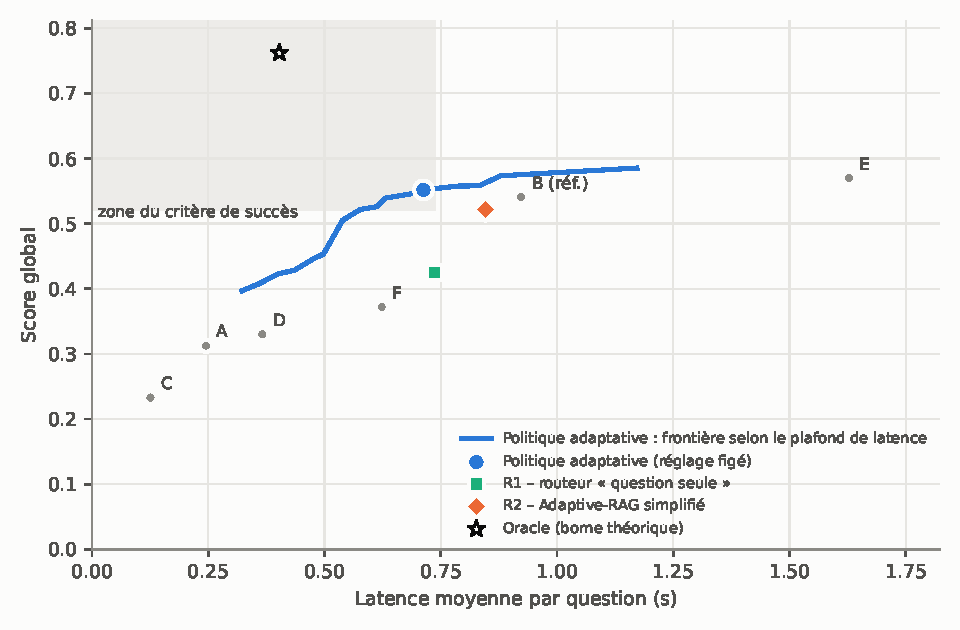
\includegraphics[width=0.9\textwidth]{figures/partie4_qualite_cout.pdf}
\caption{Compromis qualité--coût sur le jeu de développement. La courbe bleue donne, pour chaque plafond
de latence, le meilleur score atteignable par la politique ; le point bleu est le réglage figé.}
\label{fig:dev}
\end{figure}

\begin{table}[H]
\centering\small
\begin{tabular}{l c c c}
\toprule
\textbf{Catégorie} & \textbf{B} & \textbf{Politique} & \textbf{Écart} \\
\midrule
Simple       & 0,678 & 0,538 & $-14{,}0$ \\
Complexe     & 0,362 & 0,317 & $-4{,}5$ \\
Non couverte & 0,583 & 0,800 & $+21{,}7$ \\
\bottomrule
\end{tabular}
\caption{Score par catégorie (60 questions chacune), jeu de développement.}
\label{tab:categories}
\end{table}

\paragraph{Lecture.} La politique égale B en score global tout en étant 23\,\% plus rapide, et elle se
trompe moins souvent quand elle répond (risque 0,34 contre 0,39). Elle fait mieux que les deux routeurs
de référence. Ce résultat a cependant un prix clair : elle répond à moins de questions (couverture 0,48
contre 0,62). Le gain vient des questions non couvertes, où l'abstention précoce est la bonne réponse,
tandis que les questions simples perdent 14 points : la preuve BM25 classe à tort comme « faibles »
certaines questions qui ont bien une réponse. Le critère secondaire de robustesse (aucune catégorie au-delà
de 5 points de perte) n'est donc pas satisfait sur le jeu de développement.

%======================================================================
\section{Ablations}\label{sec:ablations}
%======================================================================

Chaque brique est retirée, puis la politique est réglée de nouveau sous la même contrainte de latence.

\begin{table}[H]
\centering\small
\begin{tabular}{l c c c c}
\toprule
\textbf{Variante} & \textbf{Score} & \textbf{Écart à B} & \textbf{Latence} & \textbf{Couv.} \\
\midrule
Politique complète (figée) & 0,552 & $+1{,}1$ & 0,71 s & 0,48 \\
Sans recherche adaptative (toujours 3 passages) & 0,548 & $+0{,}7$ & 0,68 s & 0,47 \\
Sans abstention finale & 0,546 & $+0{,}5$ & 0,71 s & 0,49 \\
Sans abstention précoce (meilleure cascade) & 0,395 & $-14{,}6$ & 0,71 s & 0,77 \\
Sans aucune abstention & 0,389 & $-15{,}2$ & 0,71 s & 0,80 \\
\bottomrule
\end{tabular}
\caption{Ablations sur le jeu de développement. La variante « sans cascade » est identique à la politique
complète, puisque le réglage retenu n'utilise pas la cascade.}
\label{tab:ablations}
\end{table}

\paragraph{Ce que montrent les ablations.} L'\emph{abstention précoce} porte presque tout le gain : sans
elle, aucune variante ne s'approche de B sous la contrainte de latence. La recherche complémentaire et
l'abstention finale apportent moins d'un point chacune, un écart non significatif sur 180 questions.

%======================================================================
\section{Discussion}\label{sec:discussion}
%======================================================================

\begin{itemize}
\item \textbf{La décision « faut-il répondre ? » compte plus que « quel modèle ? »}. Sous une contrainte de
latence, il est plus rentable d'éviter de générer pour les questions sans réponse que de confier les
questions faciles au petit modèle.
\item \textbf{Le petit modèle n'est pas rentable ici} : il est nettement moins bon que le grand (0,33
contre 0,54 avec 3 passages), et sa confiance ne suffit pas à repérer ses erreurs. Avec un écart de
taille de 2,7 seulement entre les deux modèles, une cascade ne paie pas.
\item \textbf{Dépendance à la composition du benchmark} : un tiers des questions sont non couvertes, et le
score global pèse les catégories à parts égales. Dans un usage où les questions sans réponse seraient
rares, l'abstention précoce rapporterait moins et coûterait davantage en couverture. Ce point devra être
discuté dans l'article.
\end{itemize}

%======================================================================
\section{Limites}\label{sec:limites}
%======================================================================

\begin{itemize}
\item Réglage et exploration sur 180 questions seulement : l'écart entre le réglage figé ($+1{,}1$) et la
validation croisée ($-2{,}1$) montre l'optimisme du premier.
\item Deux conceptions ont été essayées ; d'autres signaux (accord entre réponses, reformulation de la
question, recherche itérative) n'ont pas été explorés.
\item Le signal de preuve est lexical : il pénalise les questions dont les mots diffèrent du texte source.
\end{itemize}

\appendix
\section{Reproduire}
\begin{small}
\begin{verbatim}
HF_HUB_OFFLINE=1 python bench/run_strategies.py dev partie4   # étapes avec confiance
HF_HUB_OFFLINE=1 python bench/politique.py                    # réglage, VC, ablations
python bench/plot_partie4.py dev                              # figure
\end{verbatim}
\end{small}

\end{document}
